\subsection{Discharge Circuitry}
The discharge circuitry provides a means to determine the bulk capacitance value of the DUT from the RC time constant. Once the DUT is charged to the desired voltage, the charging relay will open and then the high-current discharge relay will close. The current through the DUT will be measured as it decays.

There are 3 switched discharge stages that allow for the decay rate to be regulated. Each stage allows for a range of voltages and capacitances needed to stay within safety and operational constraints. As seen in Figure: \ref{opArea}, there are two constraints on both the voltage and capacitance. The lowest valued resistor constrains the maximum voltage when using that stage due to its power rating. The other two stages are constrained by the overall safety limit of 500VDC. The minimum capacitance for each stage is determined by setting a requirement of at least $100$ ADC samples per time constant with a sampling rate of $250KSPS$. The maximum capacitance for each stage is determined by setting a maximum time constant.

\begin{figure}[ht!]
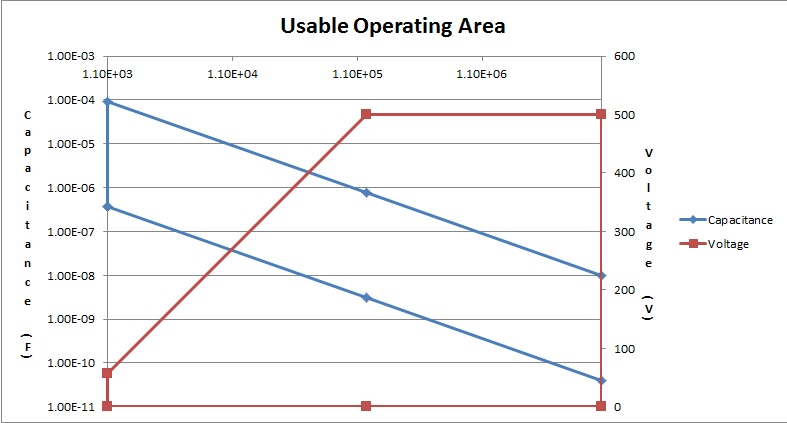
\includegraphics[keepaspectratio=true,width=3in]{./figures/circEx/operatingArea.jpg}
\centering
\caption{Operating Area}
\label{fig:opArea}
\end{figure}

